\documentclass{article}
\usepackage{style}
\begin{document}
\maketitle
\tableofcontents
\section{Introducción}
En esta práctica se implementaron los algoritmos:
\begin{itemize}
	\item \textbf{Order Crossover:} Esta técnica fue propuesta por Davis. El algoritmo es el siguiente (los padres
son P1 y P2):
	\begin{itemize}
		\item  Seleccionar (aleatoriamente) una sub-cadena P1.
		\item  Producir un hijo copiando la sub-cadena en las posiciones correspondientes
a P1. Las posiciones restantes se dejan en blanco.
		\item  Borrar los valores que ya se encuentren en la sub-cadena de P2. La secuencia resultante contiene los valores faltantes.
		\item  Colocar los valores en posiciones no conocidas del hijo de izquierda a
derecha.
		\item  Para obtener el segundo hijo, se repiten los pasos del 1 al 4, pero tomando
ahora la sub-cadena de P2.
	\end{itemize}
	\item \textbf{Partially Mapped Crossover:} Esta técnica fue propuesta por Goldberg y Lingle y tiene ciertas similitudes
	con Order Crossover.El algoritmo es el siguiente:
	\begin{enumerate}
		\item Elegir aleatoriamente dos puntos de cruza.
		\item Intercambiar estos 2 segmentos en los hijos que se generan (como la cruza
de 2 puntos convencional).
		\item El resto de las cadenas que conforman los hijos se obtienen haciendo mapeos
entre los 2 padres:
		\item Si un valor no está contenido en el segmento intercambiado, permanece
igual.
		\item Si está contenido en el segmento intercambiado, entonces se sustituye
por el valor que tenga dicho segmento en el otro padre.
	\end{enumerate}
	\item \textbf{Position-based Crossover}:Esta técnica fue propuesta por Syswerda como una adaptación de la cruza
uniforme para permutaciones. El algoritmo es el siguiente:
	\begin{enumerate}
		\item Seleccionar (al azar) un conjunto de posiciones de P1 (no necesariamente consecutivas).
		\item Producir un hijo borrando de P1 todos los valores, excepto aquéllos que
hayan sido seleccionados en el paso anterior.
		\item Borrar los valores seleccionados de P2. La secuencia resultante de valores
se usará para completar el hijo.
		\item Colocar en el hijo los valores faltantes de izquierda a derecha, de acuerdo a
la secuencia de P2.
		\item Repetir los pasos del 1 al 4, pero tomando ahora la secuencia de P2.
	\end{enumerate}
	\item \textbf{ Order-based Crossover:} Esta técnica fue propuesta por Syswerda como una ligera variante de Positionbased Crossover en la que se cambia el orden de los pasos del algoritmos.\\
	En este caso, primero seleccionamos una serie de valores de P1. Luego, removemos de P2 esos valores. A continuación generamos un hijo a partir de P2’.

	Finalmente, completamos el hijo con los valores de la secuencia obtenida de P1
(insertada de izquierda a derecha en el orden impuesto por P1).
	\item \textbf{Cycle Crossover:} Esta técnica fue propuesta por Oliver, Smith y Holland. Es similar a la
Position-based Crossover, porque toma algunos valores de un padre y selecciona los restantes del otro. La principal diferencia es que los valores tomados del
primer padre no se seleccionan al azar, sino de acuerdo a ciertas reglas específicas.\\
	\begin{enumerate}
		\item Encontrar un ciclo que se define mediante las posiciones correspondientes
de los valores entre los padres.
		\item Copiar los valores de P1 que sean parte del ciclo.
		\item Borrar de P2 los valores que estén en el ciclo.
		\item Rellenar el hijo con los valores restantes de P2 (sustituyendo de izquierda a
derecha).
		\item Repetir los pasos del 1 al 4, usando ahora P2
	\end{enumerate}
\end{itemize}
\newpage
\section{Contenido}
\subsection{Order Crossover}
\begin{figure}[h!]
	\centering
	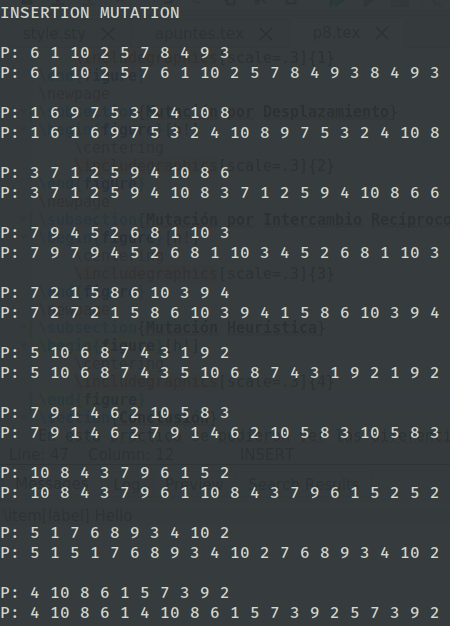
\includegraphics[scale=.3]{1}
\end{figure}
\newpage
\subsection{Partially Mapped Crossover}
\begin{figure}[h!]
	\centering
	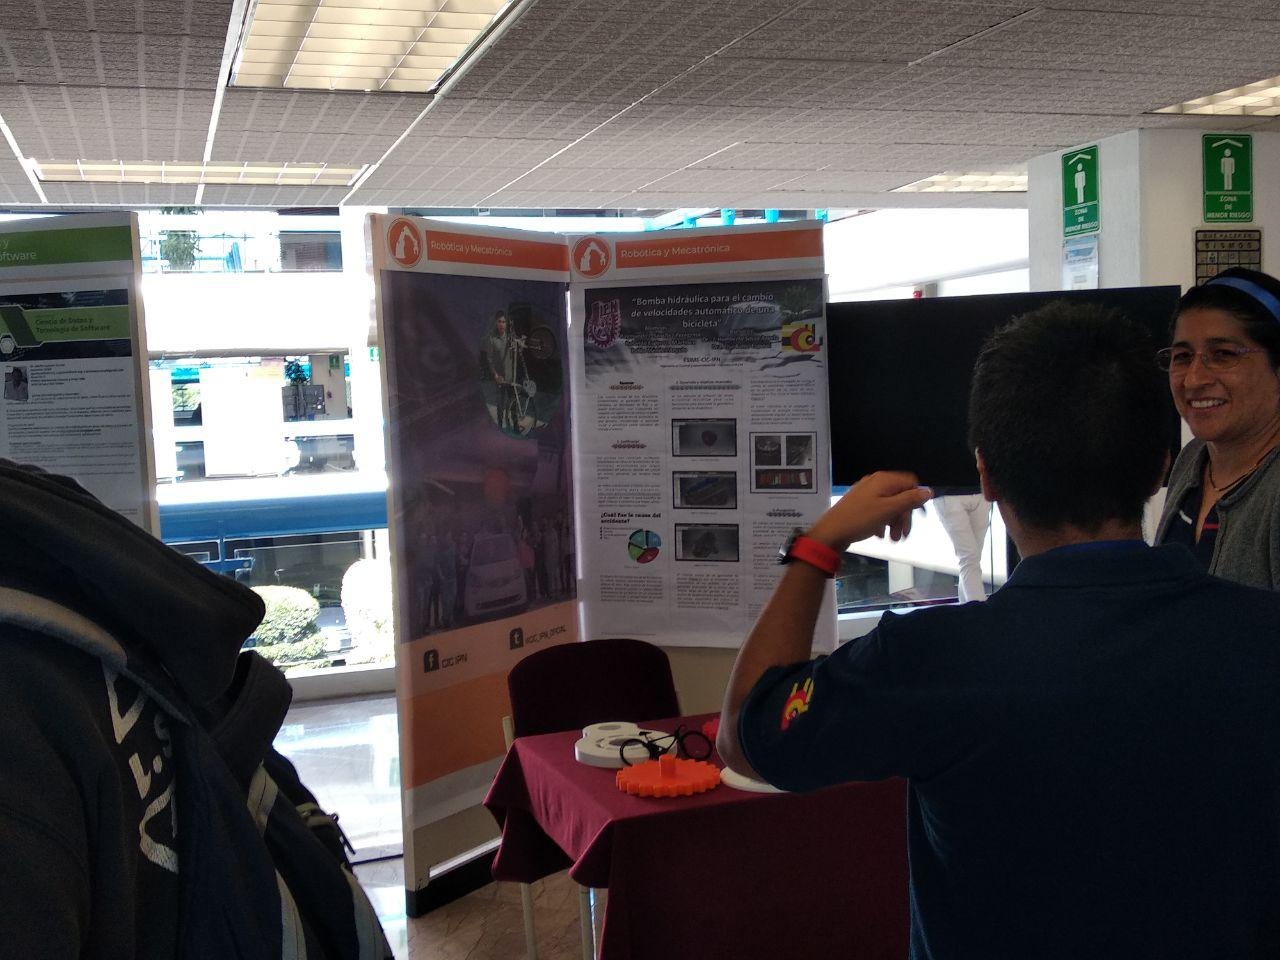
\includegraphics[scale=.3]{2}
\end{figure}
\newpage
\subsection{Position-based Crossover}
\begin{figure}[h!]
	\centering
	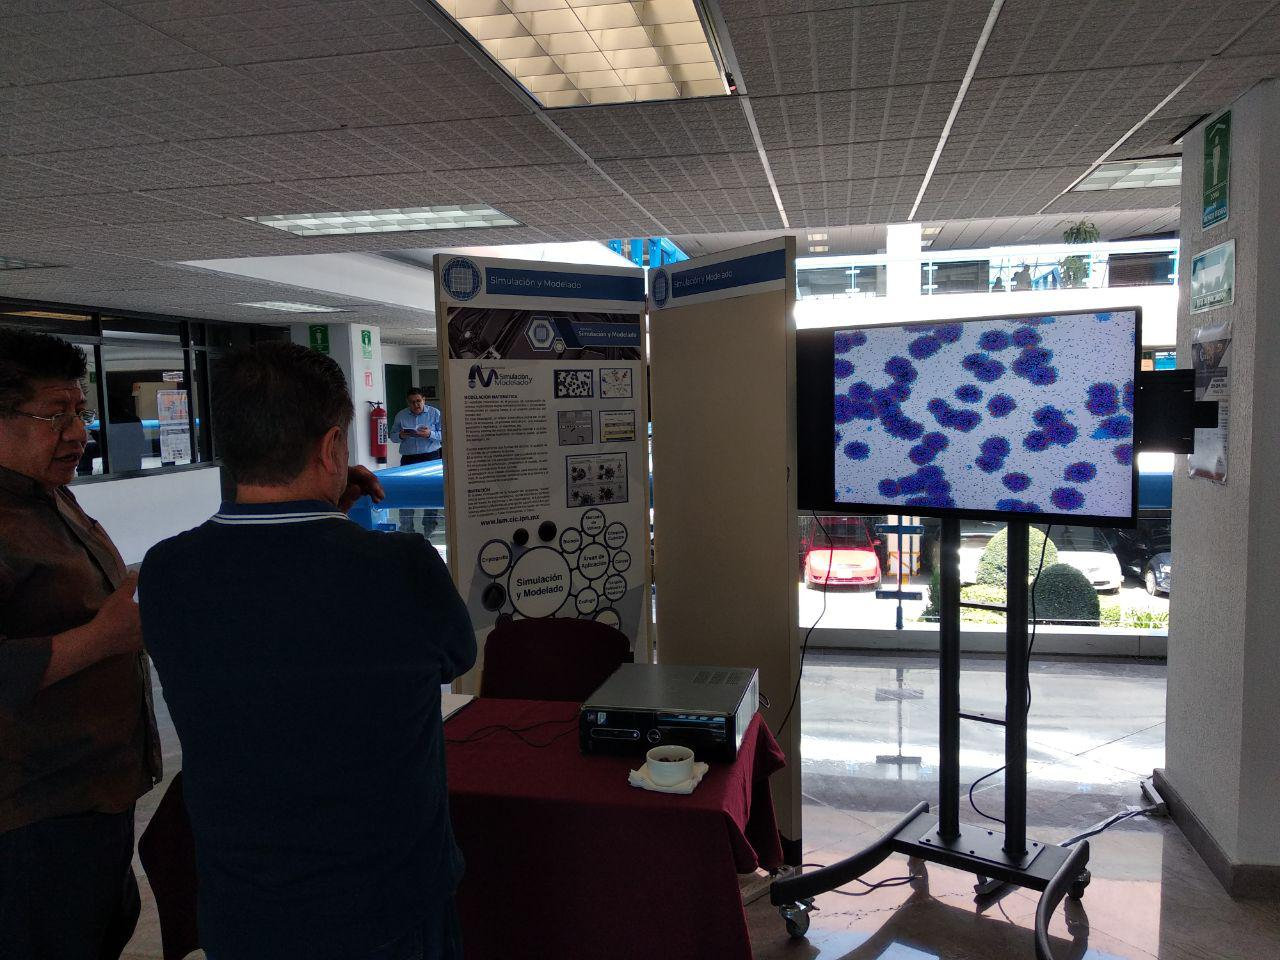
\includegraphics[scale=.3]{3}
\end{figure}
\newpage
\subsection{Order-based Crossover}
\begin{figure}[h!]
	\centering
	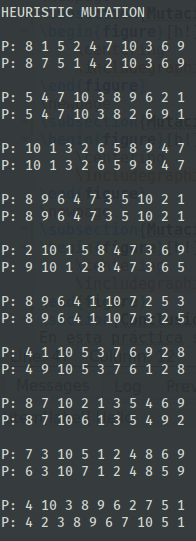
\includegraphics[scale=.3]{4}
\end{figure}
\subsection{Cycle Crossover}
\begin{figure}[h!]
	\centering
	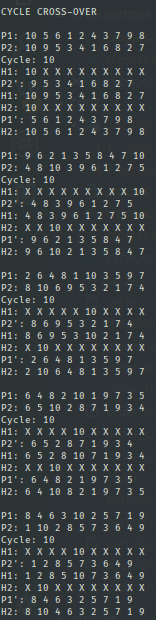
\includegraphics[scale=.3]{5}
\end{figure}
\section{Conclusión}
En esta práctica se pudieron ver las diferencias de algunos de los algoritmos más populares de cruza para permutaciones, se implementaron y se analizaron.
\end{document}